\documentclass[12pt]{article}

%% Language and font encodings
\usepackage[english]{babel}
\usepackage[utf8x]{inputenc}
\usepackage[T1]{fontenc}

%% Sets page size and margins
\usepackage[a4paper,top=2cm,bottom=2cm,left=2cm,right=2cm,marginparwidth=1.75cm]{geometry}

%% Useful packages
%\usepackage{ams}
\usepackage{amsmath}
\usepackage{graphicx}
\usepackage{tikz}
\usepackage{pgfplots}
%\usepackage{hyperref}
\usepackage[colorinlistoftodos]{todonotes}
\usepackage[colorlinks=true, allcolors=blue]{hyperref}

% table options
\usepackage{multirow}
\usepackage{arydshln}

\setlength{\dashlinedash}{0.2pt}
\setlength{\dashlinegap}{4.5pt}
\setlength{\arrayrulewidth}{0.2pt}

% bibliography shit
\usepackage{natbib}
\bibliographystyle{humannat}

\title{Using artificial intelligence to improve decision-making in conservation conflicts \\\medskip Annotated readings}
\author{Bach Adrian}

\begin{document}
\maketitle

%\newpage
\tableofcontents

\section*{Interesting sentences}
When  the  actions  of  one  party  clashes  with  the  objectives  of  another  party,  the  objectives of  one  might  be  expressed  at  the  expense  of  the  other,  causing  conservation  conflict \citep{duthie2018}.\\
Currently,  there  is  no  standard  way  to  measure  conservation  conflict  in  a  social-ecological  system  where  both the  natural  resource  (e.g.,  animals,  plants,  or  non-biological  resources)  and  the  people  (e.g.,  stakeholders,managers,  etc.)  are  modelled  in  a  single  system,  and  previous  modelling  approaches  have  not  meaningfully separated  agent  objectives  from  agent  actions. A  starting  point  to  developing  a  useful  metric of  conservation  conflict  is  to  quantify  the  deviation  of  an  individual’s  actions  from  their  objectives  (i.e.,  of actual  actions  from  desired  actions) \citep{duthie2018}.\\
GMSE  does  not  currently distinguish  female  and  male  individuals \citep{duthie2018}.\\
Conflict  might  persist  around  the  appropriate  target  population  size  rather  than  what actions  are  permitted  for  farmers;  currently,  this  potential  aspect  of  conflict  is  not  modelled,  but  future versions  of  GMSE  may  attempt  to  incorporate  such  additional  complexity  in  conflict  scenarios = Negotiations around manager's targets and policy \citep{duthie2018}.\\
Future  versions  of  GMSE  will  allow  users  to affect  one  another  directly  (representing,  e.g.,  different  groups  of  agents  lobbying  for  different  interests,among-user  conflict,  etc.) \citep{duthie2018}.\\
"No player can do better without the other player being worse off". Solutions with this property are called Pareto optimal \citep{COLYVAN20111246}. It is a solution from where the system cannot move without at least one player being worse off (includes both players being worse off).\\
If no player would unilaterally change his or her action from a solution without loosing personal outcome, it is a Nash equilibrium (supposes that the player knows what the opponent strategy is).\\
Herein lies
the real value of game theory: it provides a general and powerful
framework for analysing environmental decisions, one that
adopts a dynamical approach to decisions and naturally lends itself to an appreciation of the ongoing and far-reaching consequences of major environmental decisions. \citep{COLYVAN20111246}\\

Early  development  of  management  strategy  evaluation  (MSE)  models  originated  in  fisheries (Polacheck  et  al.,1999; Smith  et  al.,1999; Sainsbury  et  al.,2000) \citep{duthie2018}.\\

All models are wrong, but some are useful. George Box\\

Jeremy's talk (time series analyses in ConFooBio, budget optimisation and users compliance):
\begin{itemize}
    \item Assessed the quality of a strategy with the (actual, not estimated) population deviation from the manager's target.
    \item The managers' impartiality does not influence the user compliance, they do whatever they want in the limit of their budget.
    \item Engagement (involving users in the policy) increases compliance way faster and higher than enforcement (force then into doing something through pressuring their budget).
    \item  Genetic algorithm is a good candidate to model human thinking as it does not review every single possible strategies to select the best one, it selects the most fitted to its interests in a restrained population (along with discussion with Brad).
\end{itemize}
Moreover, the selection process through generations allows for stochasticity through mutation and crossing over. Hence the fittest strategy is not necessarily the optimal one, which could be interpreted as the fact that humans do not always chose the optimal option. 


\section*{Ideas}
Allow GMSE to build the world according to a GIS layer for landscape.
Include randomness into decision-making ?\\
Use impact to assess the quality of a policy?\\
Use readings to justify the need of an adaptive model such as GMSE. Given what models has been used in previous studies.\\
How to justify the strength of the causality link between management actions and resource's response.\\
Try to formalize a ConFooBio case as a game.\\
\textbf{Lit review has to present a very clear path from a large question (something like: "how modelling can help settling efficient management strategies in conservation conflicts ?") to a more specific question that will be the one I will be treating during the PhD, backed up by former studies.}\\
Be strong on the definitions of \textbf{conservation}, \textbf{conflict}, \textbf{utility}, \textbf{game} in the theoretical sense, \textbf{Nash equilibrium}, \dots\\
Emphasize on the fact that a sustainable conservation strategy is not to focus on nature only, but to find trade-offs between humans' interests and biodiversity.\\
\textbf{WHY SEEKING CONSERVATION ?}\\
Cognitive bias : anchor effect. We usually need a first guess to calibrate our judgement, but the utility associated with this guess strongly influences the way we estimate the alternative options' utility.\\
design a survey on how people perceive AI.

\subsection*{Brad meeting on 12th of october}
Lands close to public areas suffer from a higher problematic population, because resources reproduce faster in public areas. Plus, the other landowners scare theirs away. There might be a need to adapt policies to public areas proximity.\\
GMSE is implemented well enough because, following rules based on real cases observations, it succeeds in finding policies that equitably conserve the species and maintain users yield.
Even if it can not fit perfectly to all the possible situations (which is not its goal), the model can help to spot relevant aspects of the conflict that were neglected before.
It is meant to be compared to actual cases, highlighting important factors, and to provide help for decision-making, giving an idea of the long term consequences of a policy in an idealistic situation.\\
%GMSE is a decision helping tool, allowing a long term idea of the consequences of the policy. It is also useful to sort out which behaviour or which phenomenon that were not implemented in the model can make it deviate from the actual case, meaning they are worth paying attention at.
Comparing to real case studies to asses the robustness of the model would not be relevant because of the myriad of uncontrollable factors that can influence population dynamics, spatial distribution and users choices.
Plus, it's very costly.
But would be a good way to show the flexibility of GMSE, showing that it could provide a suitable strategy without the need for full knowledge of the possible sources of variation in decision-making or population dynamics.
Implementing random factor to simulate unexpected events, the fact that agents are not game theory experts, and can sometimes not choose the best option, would require an actual justification, why would it be interesting?
What question would it answer?
Note that the genetic algorithm already introduces stochasticity in the decision-making.\\
GMSE is predicted to be used by managers, or research scientists, but it could also be a way for "users" to understand why they are imposed quotas and interdiction.
Nonetheless, it would require a more friendly interface.\\
The 80 stakeholders simulation took ca 12 hours, also because the population was very large.
But it shows that the genetic algorithm could use parallelisation.\\
To show GMSE needs improvement, point at the situations where the four criteria of a successful strategy are not fulfilled. E.g : when the population is well managed but implying a broader income difference between the users. This could be a reason for the users (or the managers) to change the population target for example, should it be through negotiations.
Brad's idea: use a measure of conflict as a threshold to initiate interactions (e.g: negotiations).\\
Implementing a estimation-type-dependent population variation (estimated population and population target difference) threshold under which managers would rather not intervene at this time step, and see what happens.
Maybe allowing them to save some budget for next time step.
Good training on C. The increase in budget must be coherent with what the budget represents.
It could be a mix of money, time, energy, well-being.\\


\section{GMSE:  an  R  package  for generalised  management  strategy  evaluation - Duthie,  AB,  et al.  (2018).}

\textbf{Key words}: Conservation, conflicts, adaptive management, genetic algorithm, spatially explicit population dynamics.\\

According to GMSE framework, a satisfying management strategy implies (not in order of importance):
\begin{itemize}
    \item Equitable spatial distribution of the resource on users lands.
    \item Focal species abundance stays close enough to the manager target.
    \item Users yield reaches a satisfactory percentage.
    \item Low differences between users yields.
\end{itemize}

Basic functioning of GMSE.
\begin{enumerate}
                \item A population of discrete resources (e.g.,a managed species) with individual traits (e.g., location, age) is modelled on a spatially-explicit landscape and can simulate resource birth, movement, interaction with the landscape, and death; the discrete nature of resources causes demographic stochasticity, and therefore uncertainty. %This sub-model is unique in not relying on other sub-models because ecological dynamics can be simulated in the absence of observation and management.
                \item Observation is modelled in one of four ways: resource counting on a subset of landscape cells (e.g., Nuno et al., 2013), marking and recapturing a fixed number of resources, and resource counting across the whole landscape either one linear transect or one rectangular block at a time (during which resources might move). Sampling error from all observation types generates a range of uncertainties that depend on monitoring effort.
                \item Managers analyse data collected from observations to estimate resource abundance, then compare this estimate with their predefined target abundance. Policy is developed by calling the genetic algorithm, which works within a manager’s constraints to find costs for user actions on the resource (e.g., culling, scaring, etc.) that minimise deviation from the target abundance, as informed by the predicted consequences of each action on resource abundance and user action histories.
                \item After a suitable policy is found, users perform actions that affect resources or landscape cells. Users respond to policy individually, each calling the genetic algorithm to find actions that maximise their own utilities (e.g., maximise resource use or landscape yield) within their imposed constraints. Once each user has found an adaptive strategy, user actions affect resources and landscape cells, feeding back into the resource sub-model.
\end{enumerate}
\begin{center}
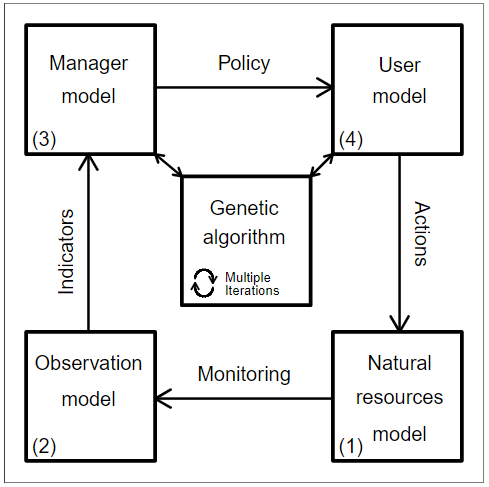
\includegraphics[scale=0.5]{GMSE-diagram.PNG}
\end{center}

Genetic algorithm: called each time a manager or a user has to make a decision. Generates a unique population of strategies (e.g. for a manager, allow such budget to such change in the cost of actions) with an associated fitness. The algorithm allow them to "\textbf{cross-over and mutate}" and reevaluates their fitness. After burning some iterations, the decision is made when the fittest strategy fitness increase is below a chosen threshold.\\

SI1:  Each  run  of  the  genetic  algorithm  mimics  the evolution  by  natural  selection  of  a  population  of  potential  manager  or  user  strategies  over  multiple  iterations.\\
Deeper in the code for ACTION arrays, the  first  column Act identifies the  type  of  action  being  performed;  a  value  of  -2  defines  a  direct  action  to  a  resource  (e.g.,  culling  of  the resource),  and  a  value  of  -1  defines  direct  action  to  a  landscape  (e.g.,  increasing  yield).  Positive  values  are currently  only  meaningful  for Manager\_Actions,  where  a  value  of  1  defines  an  action  setting  a  uniform  cost of  users’  direct  actions  on  resources  (i.e.,  costs  where Act  =  -2 for User\_1\_Actions and User\_2\_Actions). \textbf{It's a key value to add interactions between agents, e.g. a value of X is a direct action on user1 specifically)}\\
\textbf{Adding a new type of stakeholder = a new layer in ACTION array}\\
The  fitness  of  each  layer  is evaluated  based  on  how  the  layer  is  predicted  to  affect  resources  or  landscape  output  to  which  the  agent  has assigned  some  utility. \\
\textbf{Cross-over}:  each individual  selects  a  partner,  then  exchanges  corresponding  array  elements  affecting  agent  actions  (columns 8-13)  with  their  partner  at  a  fixed  probability  of ga\_crossover.\\
\textbf{Mutation}:  For  each  array  element,  a  random  uniform  number u$\in$[0,1] is  sampled.  If u is greater than 1  -  (0.5  *  ga\_mutation),  then  the  value  of  the  array  element  is  increased  by  1.  If u is  less than 0.5  *  ga\_mutation,  then  the  value  of  the  array  element  is  decreased  by  1. Increase mutation if u is close to 1, decrease mutation if very close to 0, otherwise nothing. \\
\textbf{fitness}:  Individual fitness  is  defined  by  a  real  number  that  increases  with  the  degree  to  which  an  individual’s  actions  are  predicted  to  increase  entities  of  positive  utility  and  decrease  entities  of  negative  utility.\\
\textbf{Land utility}: When land\_ownership  =  FALSE(default,modelling  users  that  harvest  resources),Uures=−1 and Uuland=  0,  and  when land\_ownership  =  TRUE, Uures=  0 and Uuland=  100(modelling  farmers  trying  to  increase  crop  yield).

Genetic algorithm is well adapted to management strategies because it's a \textit{I know it when I see it} approach. No prior knowledge of the best solution, but ability to judge the quality of a proposition and, compare it to previous ones.\\

Geese example (scare or cull): Only the estimates of population size from the observation model are available to the manager, so policy change at any time step is driven primarily by the deviation of the currently estimated population size from the manager’s target and the actions of farmers in the previous time step. Hence, when the population size is estimated to be below (above) the manager’s target, the manager increases (decreases) the cost of culling and decreases (increases) the cost of scaring. Because the manager does not know in advance how farmers will react to policy change, they assume a proportional response in total actions with respect to a change in cost (e.g., doubling the cost of culling will decrease stakeholder culling by1/2). Farmers responding to policy are interested only in minimising waterfowl’s exploitation of their crops, so they will either cull or scare to remove the waterfowl from their land, depending on which option is more effective (i.e., cheaper).\\

\textbf{Further improvement for the genetic algorithm}: Future  versions  of  GMSE  might  improve upon  these  heuristics  to  generate  more  accurate  or  more  realistic  models  of  human  decision  making.  Such improvements  could  incorporate  additional  information  such  as  memory  of  actions  from  multiple  past  time steps,  or  a  continually  updated  estimate  for  how  actions  are  predicted  to  affect  resource  abundance  or  landscape output  in  a  simulation  (e.g.,  through  a  dynamic manager\_sense).  Alternatively,  future  improvements  could usefully  incorporate  knowledge  of  human  decision  making  collected  from  empirical  observation  of  human behaviour  during  conservation  conflicts.\\  

\textbf{\texttt{gmse\_apply}}: we  can  use  it  to  study  change  in  policy  availability. E.g.  what  happens when  scaring  is  suddenly  introduced  as  a  possible  policy  option. To see  how  manager  or  user  power  changes  over  time.  If  users’  budgets  increase  by  100 every  time  step,  with  the  manager’s  budget  remaining  the  same.  The  consequence  of  this  increasing  user budget  is  higher  rates  of  culling  and  decreased  population  size.\\
To avoid crashes, when an argument that changes the data structure is added, gmse\_apply builds a new set of agents and a new world at each call.\\

The aim of GMSE is not only conservation or maximising human activity income, but to reduce the conflict in a equitable way.\\

\textbf{SI6}: GMSE  might  be  used  to  assess  the  risk  of  extinction  in  a  managed  population, through repeated simulations varying in the frequency of managers intervenes. Possibility of extinction increases exponentially with this frequency.

\subsection{Models in ecology}

\subsubsection{Theory and models in Ecology: a different perspective. (Caswell, 1988)}
\textbf{Key words}: Theoretical approach, experimental approach, models, legitimacy, critique.

Fight the unjustified criticism towards mathematical models in ecology.
Mathematical models allow the exploration of the possible patterns, which suggests "new ways of looking at problems".
Theory in biology aims at exploring the range of possible patterns in order to identify the systems boundaries ("this can happen, this cannot").
One cannot expect theory to be infallible, as any knowledge accessible to us, including experimental one, it is \textbf{conjectural}. 
Experimental approach is compulsory when testing if a theory actually applies in nature, but it cannot answer questions on the theory itself while modelling approach can. For example, when searching for the least assumptions to predict a given phenomenon.

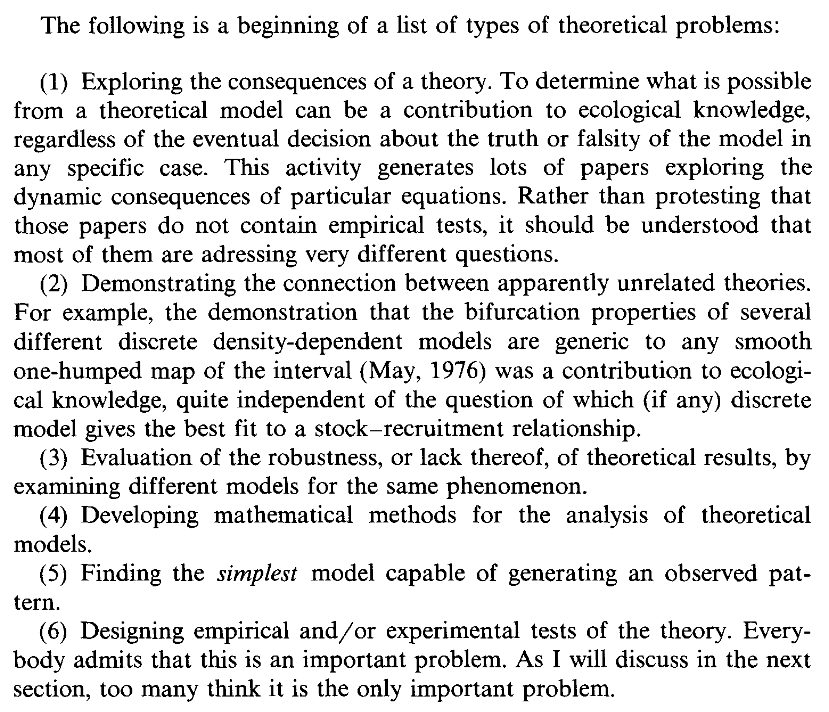
\includegraphics[scale=0.5]{theoreticalProblems1988.png}\\
\textbf{Which one is GMSE?}

Testing is not the only thing to do with theories. First, they need to be developed, and preventing people to develop theories without any backing-up data would result in slowing the discipline.\\
Refute a theory is not abandoning it, it is an encouragement for improvement.\\
"Does the model include such important factor (related to my field of study) ?". Irrelevant most of the time. Just as most experimental set-ups assessing one to two factors in relation to an other, the theoretical approach cannot take all the factors into account, and must also focus on the variables relevant to its research question.\\
\textbf{"\textit{models are to theoretical problems as experiments are to empirical problems.}"}

\section{Management strategy in conservation conflicts}

\subsection{Uncertainty and adaptive management for biodiversity conservation (Keith et al., 2011)}

(Literature review)
\textbf{Key words}: Management quality, comparative studies, role of modelling, estimated value of perfect info.

Comparative study of different strategies on the field : " Its key elements include explicit
definition of management goals, development of plausible alternative management strategies to achieve those goals, implementation of two or more strategies in a comparative experimental
framework to spread risks of management failure and improve
understanding of system responses to management, monitoring
to evaluate the relative merits and limitations of alternate strategies, and iterative modification of management strategies to improve management outcomes (Lindenmayer and Burgman, 2005)"\\
Since the response to a policy is lost into other responses from a myriad of uncontrollable external factors, monitoring the system's response to a policy over time seems not to be a good way to test and improve the policy. Also very costly! And the information gathered are most of the time estimations, that can mislead management if too far from real info. \textbf{Estimated Value of Perfect Information} can help targeting the most efficient commitment to monitoring and its scale of precision.\\
"Models are imprecise representations of complex ecological
systems, and at best can typically only predict directions of change
in response to management policies. Yet models can be extremely
useful tools that help clarify management problems and identify
important knowledge gaps that question faith in model predictions."\\
Some people implemented a way to compare different policy models in terms of learning and conservation efficiency.\\
Scientists "sometimes use policy
demands to pursue discovery goals that may never be applied to
decision making by testing their predictions. Managers often wilfully ignore scientific uncertainty to avoid complicating their message to stakeholders, and use it (or the pretence of certainty) later
when policies fail in attempts to shift responsibility for failed policy implementation to the scientific community".

\section{Game theory}

\subsection{Game Theory, Analysis of Conflict (Myerson,1997)}

\textbf{Key words}: games, utility, decision-making, cooperation, Nash equilibrium.

"\textit{Game theory can be defined as the study of mathematical models of conflict and cooperation between intelligent rational decision makers [which choices] affect one another welfare}."\\
Origins in WWII, to help understanding the issue of the nuclear cold war.\\
Games are simplified vision of actual conflicts, the actual complexity being unreachable to us. But such complexity would prevent us from understanding the fundamental issues of conflict and cooperation. As any other scientific work, game models deliberately omit less relevant details of actual situation to allow the study of particular phenomenon in the scope of a particular question.\\
Players act in order to maximise the expected value of its outcome $=$ \textit{utility}. Utility is not necessarily quantified as monetary payoff, it can be time, effort saved, well-being, happiness, and even a mix of them.\\
Players are supposed to follow the expected utility maximising theorem. This theorem is consistent with the innumerable observations of evolutionary selection in biological system, doing whatever they can to survive and/or reproduce. It can go further in terms of entropy/order, all living being tends to consume order to slow the process of entropy increasing on their body (order being the expected utility to maximise).\\
The author refers to \textit{intelligent} as players that has knowledge of the game theory framework, and is able to reach the same inferences as a game theorist. It is a questionable assumption but consistent with the fact that humans are able to learn from mistakes. (?)\\
\textit{Bayesian decision theory.} Two models for utility function: probability model (objectives unknown) and state-variable model (subjective unknowns). Objective unknowns $=$ you know the outcome possibilities and their probabilities (e.g. loteries). Subjective unknowns $=$ you do not know the probabilities (e.g. horse races).
A decision making model can be descriptive (show why a decision was the best for a player), or prescriptive (this is what you should do in this situation according to the model).\\
Several cases in which expected utility maximising is usually not respected.

\subsubsection{Models}

A model of too simple structure may miss key aspects of understanding, but a too complicated one can obscure fundamental issues.

\subsection{The conservation game (Colyvan et al., 2011)}

\textbf{Key words}: game theory, conservation conflicts, cooperation, top-down regulation, adaptive management.

Management strategy usually focuses on a single outcome, assuming a consensus on its utility among the stakeholders. In the context of conflict, such an approach is unproductive. It can be symptomatic of a certain partiality in conservation. Sustainable solution need to take all stakeholders interests into account (nature itself being also eligible as a stakeholder). Game theory framework is a better approach as it is designed to find each stakeholders actions that can lead to the best outcome for everyone.\\ 
Plus "game-theoretic perspective provides insights about: the strategies different stakeholders will likely adopt given their objectives when consensus, compromise, or cooperation are feasible; what types of cooperation best reflect stakeholder interests and achieve their objectives; which stakeholders are likely to form coalitions; the range of possible outcomes under non-cooperative and cooperative decision-making dynamics; and, whether an optimal or satisfactory solution for all stakeholders can be reached simultaneously".\\

Four main game theory examples (numbers represent gains) :
\begin{table}[ht]
    \centering
    \sffamily
    \begin{tabular}{l|r|c|c}
        \multicolumn{2}{l}{\multirow{2}{*}{}}    & \multicolumn{2}{c}{P1} \\ %\cline{3-4} 
        \multicolumn{2}{l}{}                     &      C     &     D      \\ \cline{3-4}  %\hline
        \multicolumn{1}{r}{\multirow{2}{*}{P2}} & C &     \textbf{2,2}      &      1,1     \\ \cline{2-4} 
        \multicolumn{1}{r}{}                  & D &     1,1      &     0,0      \\
    \end{tabular}
    \caption{\textit{Simple} game $=$ No costs for actions. E.g : two bordering countries cooperate for the management of a species at no cost. Both countries choosing to conserve is the highest personal gain both players can get. If one of the countries chose not to participate, personal gain is lower for both, which makes [C,C] Pareto optimal. There is no way that a player can be better off than the other by moving from [C,C], for any of the opponent strategies, the best option is always cooperation; making it also a \textbf{Nash equilibrium}.}
    \label{tab:sigam}
\end{table}
\begin{table}[ht]
    \centering
    \sffamily
    \begin{tabular}{l|r|c|c}
        \multicolumn{2}{l}{\multirow{2}{*}{}}    & \multicolumn{2}{c}{P1} \\ %\cline{3-4} 
        \multicolumn{2}{l}{}                     &      C     &     D      \\ \cline{3-4}  %\hline
        \multicolumn{1}{r}{\multirow{2}{*}{P2}} & C &     1,1      &      \textbf{1,2}     \\ \cline{2-4} 
        \multicolumn{1}{r}{}                  & D &     \textbf{2,1}      &     0,0      \\
    \end{tabular}
    \caption{\textit{Chicken} game $=$ action have a cost. E.g : two bordering countries face the problem of the management of a shared species implying costs (-1 in gain). Hence, if a party conserves and the other defects, the later enjoys some of the benefits from conservation without paying its cost, but the management is \textbf{as} efficient. Here, the system can always find a situation to move in so at least one party is better off, meaning there is no Pareto optimal situation. Knowing the other party strategy, the best outcome for a country would be [D,C], and if the situation stayed the same this country would have no reason to move away from its position. Since each party would have the same thinking, the system has two \textbf{uncorrelated Nash equilibria}.}
    \label{tab:chigam}
\end{table}
\begin{table}[ht]
    \centering
    \sffamily
    \begin{tabular}{l|r|c|c}
        \multicolumn{2}{l}{\multirow{2}{*}{}}    & \multicolumn{2}{c}{P1} \\ %\cline{3-4} 
        \multicolumn{2}{l}{}                     &      C     &     D      \\ \cline{3-4}  %\hline
        \multicolumn{1}{r}{\multirow{2}{*}{P2}} & C &     \textbf{2,2}      &      0,1     \\ \cline{2-4} 
        \multicolumn{1}{r}{}                  & D &     1,0      &     \textbf{1,1}      \\
    \end{tabular}
    \caption{\textit{Stag} game. E.g : bordering countries face the problem of the management of a shared species implying costs. The management is efficient only if all countries apply it, but countries can chose cheaper and less efficient unilateral policies. The best outcome is cooperation, which is a situation from which moving would be disadvantageous for at least one party (Pareto optimal situation). If one party cooperate, the other's best option is to cooperate as well, so (C,C) is also a Nash equilibrium. If one party defects, other's best option is to defect as well, so (D,D) is also a Nash equilibrium. Note that if countries have no information on the neighbours' policy, the best option is to defect. Also, "whether the game is chicken or a stag
hunt depends on how many countries must cooperate to achieve
the conservation goal. All countries
having to cooperate (i.e. stag hunt)
or only some countries must cooperate
(i.e. chicken)"}
    \label{tab:stagam}
\end{table}
\begin{table}[ht]
    \centering
    \sffamily
    \begin{tabular}{l|r|c|c}
        \multicolumn{2}{l}{\multirow{2}{*}{}}    & \multicolumn{2}{c}{P1} \\ %\cline{3-4} 
        \multicolumn{2}{l}{}                     &      C     &     D      \\ \cline{3-4}  %\hline
        \multicolumn{1}{r}{\multirow{2}{*}{P2}} & C &     3,3      &     0,5    \\ \cline{2-4} 
        \multicolumn{1}{r}{}                  & D &     5,0      &     \textbf{1,1}      \\
    \end{tabular}
    \caption{\textit{Prisoner} game. E.g : two bordering countries share the costs of management of a species. If one country defects, its gains increase because the species is conserved at no cost while the other pays more for the same conservation outcome. If they both defect, no money for the management and it fails, but at least no one is paying for the other's gains. Again, there is no situation from which moving would not imply one of the parties to be better off, so no Pareto optimal situation. But defecting is the best choice for any of the other country strategy, so [D,D] is a Nash equilibrium.}
    \label{tab:prigam}
\end{table}


Tendency to defect can be discouraged by applying political penalties. WE WANT TO CHANGE THE UTILITIES SO THAT COOPERATION IS A PARETO OPTIMAL NASH EQUILIBRIUM.\\
Game theory can help foreseeing the impacts of a given policy, as long as "agents [can] be explicit
about goals, strategies about the best ways to achieve those goals, monitor strategy success, and modify strategies given the impact of other agents on those goals."
"Being "self-
interested" in game theory only requires that all such considerations are fully reflected in the agent’s preference ordering."\\
The challenging part in game theory applied to conservation is to determine which type of game is being played. The various games
we are uncertain about can be represented as states of the world in
a decision problem. "Probabilities
should be assessed for each game (i.e. the probability that a particular game is being played) and expected utilities of actions are calculated by weighing outcome utilities with their respective
probabilities. If there is no chance the conservation goal can be achieved without cooperation, three
policy regime options are available: transform chicken to a simple
cooperative game, transform stag hunt to a simple cooperative
game, or do nothing. The payoffs for each regime are the summed
payoffs of the relevant games less the costs associated with the regime transformations". It takes advantages of both game and decision making theory.\\

\textbf{Tragedy of the commons} : each individual of a commons aims at maximizing its gain of the pool-resources. In this case, an individual associate a positive utility at resources assimilated, while the negative utility associated with the consummation of the pool-resources is shared upon all the commons. That way, the utility of assimilating resources is almost always greater than the negative utility of resources consummation. Therefore, if each individual acts that way, the outcome is the pool-resources depletion. Solution : third party imposes limits to individuals, implementing sanctions with negative utility compensating the utility of individual pool-resources over-consumption (\textbf{top down regulation}).\\
"Empirical studies show that in many conservation contexts
cooperation is more likely to emerge from bottom-up community-based programs than top-down enforced regulation".\\
"The extant incentive structure only targets individual hunters
through punishment rather than benefits, while non-hunters reap
tangible rewards from a successful wildlife management program—the consequence is that hunters reject the management regime."\\
‘‘no self-monitoring agreement can be sustainable without a payment to each individual that exceeds the opportunity cost of monitoring—even if no one is poaching’’ (
Mesterton-Gibbons and
Milner-Gulland, 1998).\\
"i) fines proportional to the number of trophies in a poacher’s
possession are more effective than fixed fines, (ii) increasing the effort devoted to detecting and prosecuting poachers is more effective than increasing the severity of punishment to poachers" and (iii) the success of bans on international ivory trade is ambiguous, depending on the assumptions in
the model. The fact that banning ivory could increase elephant
poaching is particularly interesting. It could be caused, at least in
part, by an expected rise in ivory prices that would enhance incentives to poach elephants (from review by Keane et al., 2008). Also, trade bans can accelerate species toward
extinction if speculators bet on future price increases by \textbf{stockpiling}, with the intention of cashing in on their stock once the species
becomes extinct.\\

"oversimplification is assuming that nature’s response is straightforward and easily predictable following conservation actions such as monitoring or managing species." (marking bias as an example). Indeed, how to justify the strength of the causality link between management actions and resource's response.
"representing nature as part of the fixed background structure of the
conservation problem is inaccurate. Rather, it should be treated
as another player in the game."\\
Other assumptions in games : "they are perfectly rational
expected utility maximisers (ndlr. - is it the case for nature as a player ?) [...] [which] require players be expert game theorists: they must know
not only what their strategy should be, but also what other players’
strategies should be." It is already a questionable assumption for human, but for "nature", which is not supposed to be conscious nor rational -\textbf{IS IT ?}-, it is even more "implausible".\\
But you could model "nature" as a player like : "In hydrology, for example, nature
can be represented as an agent that prefers liquids to attain their
lowest level of energy and it schemes to make this happen. Humans attempting to increase water tables or construct artificial lakes are players
with different intentions and they must play against nature."\\
"It is useful to distinguish between nature as a player in a game
and nature as a rule maker. There will be structural features of the
game —such as, which moves are available to a player— that are
immutable and non-negotiable." It can also play both roles, just as a government that sets costs (rule-maker, manager), but is open to negotiations (player).\\
"a core conservation
concern: ensuring species (and environmental resources more generally) never reach irreversible thresholds below which population
decline and ultimate extinction are inevitable." Such a concept was argued for a lack of empirical validation, and uncertainty in prediction. But it also does not include insights of the economical value a resource can have to humans.\\

"How the game is represented significantly affects what conservation actions are defensible and/or whether a compelling rationale for conservation exists."

"Herein lies
the real value of game theory: it provides a general and powerful
framework for analysing environmental decisions, one that
adopts a dynamical approach to decisions and naturally lends itself to an appreciation of the ongoing and far-reaching consequences of major environmental decisions."

\section{Decision-making}

\section{Artificial intelligence}

\subsection{Genetic algorithms}

\section{Why should we conserve? From an evolutionary point of view.}
Caution! Use more conditional mode.\\
Does conservation make sense?
Why do we want it?\\
The scientific/ecological reasons:
\begin{itemize}
    \item Biodiversity is necessary for the maintain of the ecological balance (we depend on).
    \item It fuels evolution.
    \item We strongly depend on environmental services (pollination, CO2 absorption, maintain of soil, bio-degradation, soil maintenance, and many more), that might be affected by losses of biodiversity. 
    \item Biodiversity insure a quick and adapted response to change. Some of which are useful to us (lots of cure molecules were discovered thank to species that already used it).
    \item Source of inspiration through biomimetism.
    \item \dots
\end{itemize}
The ("non-scientific") non-ecology-related reasons:
\begin{itemize}
    \item We like the way nature looks, \textbf{we do not want it to change}, we want it to stay the way we used to know it.
    \item We want to leave a beautiful world to our offspring, at least as beautiful as ours. \textbf{Beautiful or just suitable?.} Interestingly, this could be interpreted as an evolutionary-driven behaviour; we were successful in that environment, we assume that our descendants are more likely to be as successful in the same environment. The chances are lower if the environment changes too much, or faster than they can adapt to.
    \item It might be a simple intent to indirectly conserve our species, because we rely on a healthy environment.
    \item We like having some species around, because they are cute or directly useful to us.
    \item It gives us an ethical purpose. We feel better trying to act on it, a sort of compensation for us being at the origin of the problem. Would any other species do that?
    \item Could also be a simple scientific curiosity for the topic. Which would be more understandable than any other reason to me.
    \item Being in control of one's environment seems satisfying to us, it is a feel of power.
\end{itemize}

Luc after someone's response at the lab drink: "Is that a satisfactory answer to your question? We conserve because we want to."
From the game-theoretic point of view, most people value (associate a positive utility to) the fact of having access to nature. They also value certain "sexy species".
But most of them also despise some aspects of the biodiversity that goes with it (insects, weed plants), and would rather not have them around (negative utility).

We might also be preventing species from evolving by maintaining their environment in a relatively steady state, thus slowing the adaptation process, getting on "its" way.

Being a pro-conservation has became the norm in "developed" countries, and anyone that would think otherwise might be ostracised.
(Same with feminism, I believe going against it, or not being aware of the problem, will significantly reduce chances to seduce a girl.)
It became a must-have to be part of a "northern modern society".
Being aware of it, seeing it as a concern, is seen as a positive signal by the community.

If it was actually/strictly environmentally-driven, it would be quite paradoxical because we are, very likely, the source of unprecedented perturbations in the ecosystem(s).
Through conservation, we extend our time spent on Earth, and delay our population drop/the natural control of our population. 
(Are we living above our carrying capacity? Probably, because it's a known fact that one planet is not enough to sustain 7 billions people living the northern way of life.)
But does it makes sense for species to embrace its own population control? We could avoid extinction, just by conserving ourselves the way we do with other species.
It is controversial, we don't mind letting farmers shoot geese when managers judge it necessary, but would we let that happen on our own species?
\textbf{Are we legitimate to act on the conservation of any species, knowing that we are not willing to deal with the initial issue which is our life style?}

A typical answer would be "it would be worse if we do nothing", but is that a correct thinking?
The dynamic and complexity of ecosystems are unreachable for our minds, or machines, who knows what could be the actual outcome of such species going extinct.
Extinctions and emergence of new species is a well established cycle, it would be interesting to see at which rate species are disappearing and emerging, and to investigate the link with human activity.
It would also be interesting to see in which group has which rate and if it changed since our "development".
Seems very tough, given that our methods have and are evolving.
Would it make sense in the way that general, overall biodiversity is not the goal of conservation, but biodiversity inside all the different "functional" groups.

Biodiversity, as the net between ecosystems, species and genetic diversities, is the key for environment to respond to change, and subsist. Losses in any kind of theses bio-diversities, or the links between them, will result in a environment much more sensible/weaker to changes.

\section{AI ethics}
\newpage
\bibliography{PhD-litReview}
\nocite{*}
\end{document}
